\documentclass[../main.tex]{subfiles}

\graphicspath{{pictures/}{../pictures/}}

\chapterimage{chapter_head_2.pdf} % Chapter heading image

\begin{document}
	\chapter{Basic Syntax}
	
	%----------------------------------------------------------------------------------------
	%	Basic Syntax
	%----------------------------------------------------------------------------------------
	
	\section{Types}
	
	Much of programming is about the receiving, manipulating, and sending of data.  Since C is a typed language, it needs to know how to interpret the data that you are working with.  In many cases, the underlying bits that are actually being stored are the same.  However, based on the type assigned to that data, the C compiler will interpret it differently.  C can't really tell the difference between 41 and the letter 'A' (which has the ASCII value of 41).  Its up to you as the programmer to specify if the data is an integer or if its a character.
	
	Below are a few of the basic data types you'll encounter in C.	
	\begin{itemize}
		\item \textbf{int}		-	Represents whole numbers.
		\item \textbf{char}		-	Represents a single character.
		\item \textbf{float}	-	Represents numbers with decimal points (single precision).
		\item \textbf{double} 	-	Represents numbers with decimal points (double precision).
	\end{itemize}

	The platform that a program is compiled for can affect the number of bytes that a data type requires.  While most of today's platforms are 64-bit, there are still a few 32-bit systems out there.  If the max or min size of a data type is a concern to you, you'll want to be sure you know the size of that type on the platform your code will be compiled for.
	%----------------------------------------------------------------------------------------
	%	Integer
	%----------------------------------------------------------------------------------------	
	\subsection{Integers}
	
	By default, an \textit{int}\index{int} utilizes 4 bytes on both the 32-bit and 64-bit platforms. However, there are a couple of qualifiers that can affect how the data is interpreted as well as how many bytes are used.  
	\begin{itemize}
		\item \textbf{short}\index{short}	-	Utilizes 2 bytes (16 bits).
		\item \textbf{long}\index{long int}		-	Utilizes 4 bytes on a 32 bit platform and 8 bytes on a 64 bit platform.
		\item \textbf{long long}\index{long long int}-	Utilizes 8 bytes on a 32 bit platform and 8 bytes on a 64 bit platform.
		\item \textbf{signed}	-	Integers are \textit{signed} by default meaning they utilize two's complement to represent positive and negative numbers.  You do not need to specify \textit{signed} but can for greater clarity for someone reading your code.
		\item \textbf{unsigned}	-	As an \textit{unsigned} integer, there is no sign bit.  Therefore you can store larger positive numbers but you cannot store negative numbers.\\
	\end{itemize}
	
	\lstinputlisting[caption={\lstname}]{src/02-integer-32bit.c}
	
	\begin{lstlisting}[language=bash, numbers=none]
		$ file 02-integer-32bit
		02-integer-32bit: ELF 32-bit LSB shared object, Intel 80386
		
		$ ./02-integer-32bit 
		Number of Bytes:
		short int: 2
		int: 4
		long int: 4
		long long int: 8
		
		Value of signed   short: -275
		Value of unsigned short: 65261
		
		Min signed int: -2147483648
		Max signed int: 2147483647
		
		Min unsigned int: 0
		Max unsigned int: 4294967295
	\end{lstlisting}
	
	As you can see with the \textit{file} command, 02-integer-32bit has been compiled as a 32-bit binary.  Notice that an \textit{int} and \textit{long int} are both 4 bytes but a \textit{long long int} is 8 bytes.  
	
	Also notice on line 11 that I assign the value of -275 to \textit{si} which is a \textit{signed short int} and it prints out just fine on line 14.  However, when I print it out a second time on line 15 I cast it as an \textit{unsigned short int}.  Under the hood, the bits haven't changed; how they were interpreted did.  -275 is actually 1111111011101101 in binary.  The left-most bit (most significant bit) is the \textit{sign} bit.  When cast as an \textit{unsigned short int}, this bit is not longer interpreted as a signed bit which is why we now get a positive number.  I point this out only because it is important to note that you as the programmer need to understand the data you are working with because C only pays attention to whether or not you declared it as \textit{signed}\index{signed} or \textit{unsigned}\index{unsigned}.  To further demonstrate this, I've printed out the max and min value that a signed integer and an unsigned integer can hold.\\
	
	\lstinputlisting[caption={\lstname}]{src/02-integer-64bit.c}
	
	\begin{lstlisting}[language=bash, numbers=none]
	$ file 02-integer-64bit
	02-integer-64bit: ELF 64-bit LSB shared object, x86-64
	
	$ ./02-integer-64bit 
	Number of Bytes:
	short int: 2
	int: 4
	long int: 8
	long long int: 8
	\end{lstlisting}
	
	Notice this 02-integer-64bit is compiled as a 64-bit executable.  In this case, an \textit{int} is still 4 bytes but a \textit{long int} is now 8 bytes allowing you to store much larger numbers.  
	
	\subsubsection{stdint.h}
	
	The \textit{stdint.h} header imports other header files such as \textit{stdint-intn.h} and \textit{stdint-uintn.h} that specify a number of macros and type definitions (\textit{typedef}) to make working with integers more consistent across 32-bit and 64-bit platforms.  By using it, you can guarantee the size of the resulting integer. 
	\begin{itemize}
		\item \textbf{uint8\_t}, \textbf{uint16\_t}, \textbf{uint32\_t}, \textbf{uint64\_t} - All unsigned integers that utilize 8-bit, 16-bit, 32-bit, and 64-bit accordingly.
		\item \textbf{int8\_t}, \textbf{int16\_t}, \textbf{int32\_t}, \textbf{int64\_t} - All signed integers that utilize 8-bit, 16-bit, 32-bit, and 64-bit accordingly.
	\end{itemize}

	Due to the inconsistent sizes for integers we identified between 32-bit and 64-bit platforms, you'll often see code that uses the \textit{stdint.h} header file and specifies the actual size that is needed.  
	
	Additionally, \textit{stdint.h} also specifies macros for the MAX and MIN sizes of various integers.  You may decide to use these in your programs to test for an overflow of an integer.
	
	\begin{verbatim}
	/* Minimum of signed integral types.  */
	# define INT8_MIN               (-128)
	# define INT16_MIN              (-32767-1)
	# define INT32_MIN              (-2147483647-1)
	# define INT64_MIN              (-__INT64_C(9223372036854775807)-1)
	/* Maximum of signed integral types.  */
	# define INT8_MAX               (127)
	# define INT16_MAX              (32767)
	# define INT32_MAX              (2147483647)
	# define INT64_MAX              (__INT64_C(9223372036854775807))
	
	/* Maximum of unsigned integral types.  */
	# define UINT8_MAX              (255)
	# define UINT16_MAX             (65535)
	# define UINT32_MAX             (4294967295U)
	# define UINT64_MAX             (__UINT64_C(18446744073709551615))
	\end{verbatim}
	
	
	%----------------------------------------------------------------------------------------
	%	Characters
	%----------------------------------------------------------------------------------------

	\subsection{Characters}
	
	A \textit{char}\index{char} within C typically requires just a single byte to store a single character.  This is based upon the fact that the \textit{char} was meant to store the ASCII\index{ASCII} value which only required 7 bits.  Depending upon the type of project you are working on, this may or may not be sufficient. Below is the ASCII chart \ref{fig:ascii} as printed out by running the \textit{ascii} command on the terminal.  Notice the values only go upto 127.
	
	\begin{figure}[h]
		\centering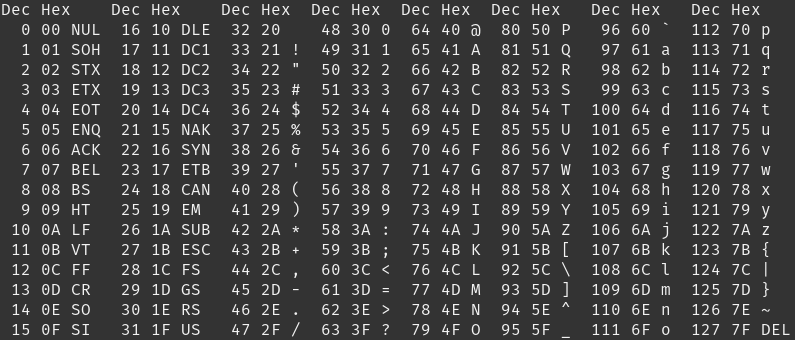
\includegraphics[scale=0.5]{ascii.png}
		\caption{ASCII Chart}
		\label{fig:ascii} % Unique label used for referencing the figure in-text
	\end{figure}
	
	Obviously the ASCII chart was built for the English language.  When not sufficient, there are ways of using an \textit{unsigned int} and \textit{UTF-8} encoding instead.  Additionally, there are wider character data types such as \textit{wchar\_t} that utilize more than 1 byte in order to store character values by their Unicode value rather than an ASCII value.  I will not be going into these methods and alternate data types but if it interests you, I suggest checking out articles such as \href{https://www.cprogramming.com/tutorial/unicode.html}{https://www.cprogramming.com/tutorial/unicode.html}.\\
	
	\lstinputlisting[caption={\lstname}]{src/02-character1.c}
	
	\textbf{Line 2}: Here I import \textit{ctype.h}.  Doing so gives me access to a number of functions and macros pertaining to the use of characters.\\
	\textbf{Line 7}: Here I declare a \textit{char} and give it the value of \textit{a}.  Notice it holds a single character and I use single quotes.\\
	\textbf{Line 8}: Here I use the function toupper which has a function \textit{declaration} of \textbf{int toupper(int c);}.  This is our first indication that under the hood, a \textit{char} is treated very much like an \textit{int}.\\
	\textbf{Line 14}: Here I use the function \textit{isalpha} to test to see if the character is alphabetic.\\
	\textbf{Line 22}: Here I use the function \textit{isdigit} to test to see if the character is a digit.\\
	
	By typing '\texttt{man 3 toupper}' on the terminal, I am presented with the manual page describing the C \textit{toupper} function:\\
	
	\begin{figure}[h]
		\centering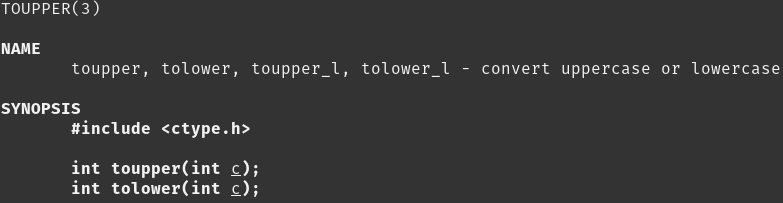
\includegraphics[scale=0.5]{toupper.png}
		\caption{toupper}
		\label{fig:toupper} % Unique label used for referencing the figure in-text
	\end{figure}

	Likewise, I can view the manpage for \textit{isdigit} by typing '\texttt{man 3 isdigit}'.\\
	
	\begin{figure}[h]
		\centering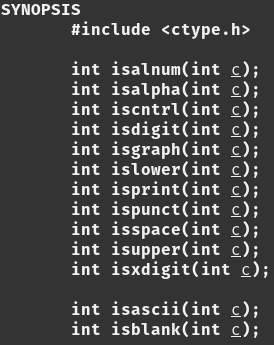
\includegraphics[scale=0.5]{isalpha.png}
		\caption{isalpha, isdigit}
		\label{fig:isapha} % Unique label used for referencing the figure in-text
	\end{figure}

	\subsubsection{Character Constants}\index{character constant}
	
	A character constant is any character surrounded by single quotes.  For example, when we assigned 'a' to \textit{c1} in the previous example, that was an example of a character constant.  However, if we were using wider characters other than the standard \textit{char}, we may want to pass in the Unicode value.  To do this we may specify \textit{u'$\textbackslash$x3b3'}\cite{c_nutshell}.    
	
	The \textit{\textbackslash} we just saw with \textit{$\textbackslash$x} known as an escape sequence.  There are a number of other escape sequences you may encounter.  You've already seen me use '\textit{$\textbackslash$n}' int nearly every \textit{printf}.  This is a character constant for the newline character.  Some of the other character constants you may encounter are:
	\begin{itemize}
		\item \textbf{$\textbackslash$0}	- The NULL character.  You'll often see this as terminating a character array.
		\item \textbf{$\textbackslash$n}	- New line.
		\item \textbf{$\textbackslash$r}	- Carriage return.
		\item \textbf{$\textbackslash$t} 	- Horizontal tab.
		\item \textbf{$\textbackslash$v}	- Vertical tab.
		\item \textbf{$\textbackslash$o}	- Octal values.  This will look something like \textit{$\textbackslash$o456} where we are referring to octal value 456 which is 302 in decimal.
		\item \textbf{$\textbackslash$x}	- Hexidecimal values.  This will look something like \textit{$\textbackslash$x456} where we are referring to hexadecimal 456 which is 1110 in decimal.
		\item \textbf{$\textbackslash$u}	- Unicode values.	
	\end{itemize}

	%----------------------------------------------------------------------------------------
	%	Floats
	%----------------------------------------------------------------------------------------
	
	\subsection{Floats}
	
	Floating point numbers are numbers with decimal points.  Just as with integers, the data type affects the number of bytes used to store values.  With integers, concern was with max and min values as well as overflows.  With floats, its about precision.  A floating point value is an approximation and the cost of being more precise in that approximation is in the number of bytes that are required to store it.
	
	Below is a chart directly taken from the book "C in a Nutshell"\cite{c_nutshell}.
	\begin{table}[h]
		\centering
		\begin{tabular}{l l l l l}
			\toprule
			\textbf{Type} & \textbf{Storage Size} & \textbf{Value Range} & \textbf{Smallest positive Value} & \textbf{Precision}\\
			\midrule
			float\index{float} & 4 bytes & $\pm$3.4$\epsilon$+38 & 1.2$\epsilon$-38 & 6 digits \\
			double\index{double} & 8 bytes & $\pm$1.7$\epsilon$+308 & 2.3$\epsilon$-308 & 15 digits \\
			long double\index{long double} & 10 bytes & $\pm$1.1$\epsilon$+4932 & 3.4$\epsilon$-4932 & 19 digits \\
			\bottomrule
		\end{tabular}
		\caption{Real floating-point types}
		\label{tab:floating-point} % Unique label used for referencing the table in-text
	\end{table}

	\lstinputlisting[caption={\lstname}]{src/02-float1.c}
	
	\begin{lstlisting}[language=bash, numbers=none]
		$ ./02-float1 
		1 / 3 = 0.000000
		1 / 3 = 0.333333
	\end{lstlisting}
	
	\textbf{Line 7}: On this line, 1 is divided by 3 and the results are stored in \textit{x}.  However, when \textit{x} is printed out on line 8, we see that what actually got stored is 0.0.  This is because we divided one integer by another integer.  In C, this will result in another integer.  Since integers cannot have decimal points, 0 gets stored in X.\\
	\textbf{Line 10}: Again we do the same division but instead of dividing two integers, we first cast 1 as a \textit{float}.  Under the hood, this operation should result in a \textit{double} being generated but because we are storing it in a \textit{floatmathmatical}, it it rounded to 6 digits of precision.  We can see this when we print \textit{x} on line 11 in that there are only 6 digits (leading and trailing zeros are ignored).
	
	There is another header file called \textit{complex.h} that allows for the use of complex floating point types.  I will not be discussing them here.
	
	\clearpage
	%----------------------------------------------------------------------------------------
	%	Mathmatical Operations
	%----------------------------------------------------------------------------------------	
	\section{Operators}
	
	The following operators are some of the most common you'll see when writing C.  
	
	\begin{table}[h]
		\centering
		\begin{tabular}{l l l}
			\toprule
			\textbf{Operator} & \textbf{Purpose} & \textbf{example}\\
			\midrule
			* 	& Multiplication 	& a * b \\
			/ 	& Division 			& a / b \\
			+ 	& Addition 			& a + b \\
			- 	& Subtraction 		& a - b \\
			\% 	& Modulus (remainder) & a \% b \\
			++ 	& Increment 		& ++a or a++ \\
			\verb|--| & Decrement 	& \verb|--|a or a\verb|--| \\
			\& 	& BITWISE AND 		& a \& b \\
			| 	& BITWISE OR 		& a | b \\
			\textasciicircum 	& BITWISE XOR 		& a \textasciicircum b \\
			\textasciitilde 	& BITWISE NOT 		& $\textasciitilde$a \\
			<< 	& Left Shift 		& a << 2 \\
			>> 	& Right Shift 		& a >> 2 \\
			= 	& Assignment 		& c = a + b \\
			==	& Equality 			& a == b \\
			<	& Less than			& a < b \\
			>	& Greater than		& a > b \\
			<=	& Less than or equal to & a <= b \\
			>=	& Greater than or equal to & a >= b \\
			!	& Negation (NOT)	& !a \\
			\&\&& Logical AND		& a \&\& b \\
			|| 	& Logical OR		& a || b \\
			\&	& Address of		& \&a \\
			*	& Indirection		& *a \\
			{[ ]}	& Subscript		& a[b] \\
			.	& Struct or Union member designator & a.b \\
			->	& Struct or Union member designator by Reference & a->b \\
			?:	& Conditional Evaluation & a ? b : c \\
			\bottomrule
		\end{tabular}
		\caption{Operators}
		\label{tab:operators}
	\end{table}

	The Assignment '=' operator is often combined with other operators such as '+', '-', '/', ' to shorten the amount of code the programmer has to type.  For example, \texttt{a += 5;} is equivalent to \texttt{a = a + 5;}.
	
	
\end{document}